\section{The Operative Year and the Method of Fractions.}

After outlining the particular characteristics of the overall chronocrators and those of the shorter time periods, I must now speak about the operative year and matters associated with it—but first it is necessary to speak a few words about those who have written on these topics. 

Most have expounded their views on the distribution of the chronocratorships in a very complicated and hateful manner, and they have not taught
a valid system. They have fenced in this topic with many devices, and have left their readers a legacy of the greatest error and of futile investigation. Others, carried away in their ignorance by this mass of words, \textbf{/172K/} have added false systems and have deceived many. Still others, who saw the power of this science and who laid a foundation, did not add examples, because of their grudging spirit. We, however, traversed many lands \textbf{/163P/} and came to Egypt, where we fell in with avaricious teachers. We paid them money because of our enthusiasm for the work, but we did not come upon the truth. So, choosing an ascetic and independent life, we occupied ourselves with other matters. But this problem of concern to the greatest of the mathematical sciences, viz. the distribution of the overall chronocratorships, drew us back and made our enthusiasm greater, and we came to consider an detailed treatment of the topic a necessity.

\index{Valen's admonition}
Since quarrels have arisen about the general method of distributing—some using the method of following the sequence of terms, others using the minimum periods, others using the dodekatemoria (which total 10 years 9 months), others using the exaltations, all of which methods of distribution falsify the results—I thought it disgraceful to limit forecasts to “year 2” or “year 10” or “year 7,” and I thought it best to investigate the chronocratorship for any year or part of a year. As a result, we have spent much time in painful labor, we have considered in painstaking detail the effects of the changing of places, and we have made experiments in close association with those who are eager for such knowledge. Eventually God of his own accord, through his providence, made clear the transmission to a given place, <giving this knowledge> through the help of a learned man. We received this as a basis, we added much labor, and we gained our goal, which we now possess, having ourselves added many useful procedures. For it is from our daily experiences, from the contributions of many men, and from our personal acquaintance with syndromes that we have compiled our divinely-inspired and immortal theorems, and we have shared them without stint, since this topic seems to be the most essential prerequisite for the remaining parts <of astrology>. Without it there neither is nor will be anything; it contains the foreknowledge of the beginning and the end. I adjure you, my most precious brother, and you, initiates into this mystic art, by the starry vault of heaven and by the twelve-fold circle, by the \Sun, the \Moon, and the five wandering stars by whom all of life is guided, and by Providence itself and \textbf{/173K/} Holy Fate, to preserve these matters in secret and not to share them with the vulgar, but only with those worthy of them and able to preserve and requite them as they deserve. I adjure you to bestow on me, Valens, your guide, eternal and noble fame, particularly since you are aware that I alone ungrudgingly illuminated this part of the truth which had never before been explicated by anyone. Do not put aside my name and attach another’s to this compendium. Do not blot out any of what has been \textbf{/164P/} or will be written here, with the result of nullifying my readers’ efforts and of bringing discredit on me. May the previously mentioned gods be well-disposed to those who guard these things: may their lives be prosperous, and may the consummation of their plans be as they wish. May the opposite happen to those who foreswear this oath: may the earth not be passable, the sea not be sailable, may they have no offspring of children, may their minds be blind and fettered, and may they lead shameful and unsuccessful lives. If after death there is a recompense for good or evil deeds, may they suffer the same there also.

Therefore, if after learning the doctrines taught here, anyone finds this system mysteriously set forth in another treatise, he must not award praise to that treatise, but he must show gratitude to us as not only the reporter but also the discoverer of many things and the perfecter of the system—for many men receive directions without stint, but give them grudgingly. Therefore I encourage those who have just met with this compendium, who are just entering the heavenly places, who are surveying for a time the dancing places and the mysteries of the gods, and who are gaining god-like glory—these I urge to lay aside the many schemes of systems and books, to become proficient in the scientific, tabulated theorems of the stars and signs and in the operations which use the tables of visible motions, and to stick to these methods which have already been prescribed. I urge them to
observe the position of the stars in degrees when necessary for determinations to the degree, to observe their positions by sign when that level of accuracy is appropriate, so that what is said will have been said truly. (Often I myself have noticed that a star is in one sign with respect to the temporal determination of transits, but in another sign with respect to visible motion, especially if the star is at the beginning or end of a sign. The same variations are possible at stationary points and at opposition to the \Sun.) Consequently, it is necessary to make the determination <of the chronocrator> only after first discovering in which signs or degrees the stars—and particularly the Ascendant—are located.

\index{distribution!profection}
\textbf{/174K/} Let us start our exposition from this point: when investigating the current year of a nativity, we divide by 12. Count the remainder from a star which is able <to transmit> to a star which is able to receive. In this way we will discover to what sign the year transmits. What I have said is easy to comprehend but complicated to determine since all the stars, plus the Ascendant, the \Sun, and the \Moon,
can transmit to and receive from each other. \textbf{/165P/} 

Let us take an example so that we may make an intelligent beginning: \Sun, \Mercury\xspace in \Aquarius, \Moon\xspace in \Scorpio, \Saturn\xspace in \Cancer, \Jupiter\xspace in \Libra, \Venus in \Capricorn, \Mars, Ascendant in \Virgo
\footnote{\textit{Greek Horoscopes} dates the chart (L120) to approximately February 8, 120AD (p.116). Also used in Book II, section 30.}.

\clearpage
\begin{wrapfigure}[15]{R}{7cm}
\centering
\vspace{-20pt}
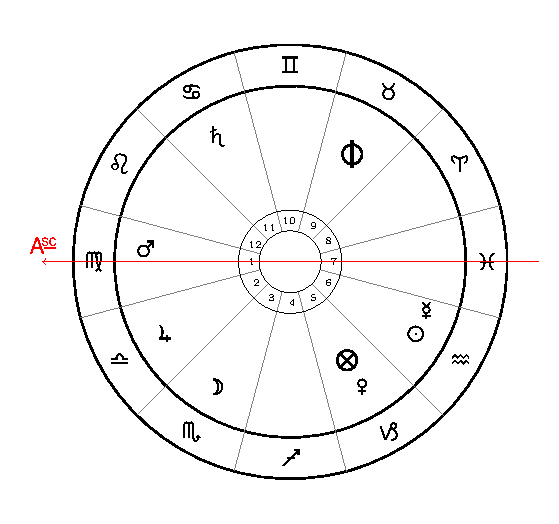
\includegraphics[width=0.68\textwidth]{charts/4_11_1}
\caption{Chart 19a [IV.11.1, GH L120]}
\label{fig:chart19a}
\end{wrapfigure} 

We are investigating the 35th year. I divide <35> by 12,
for a result of 24, remainder 11. We note which stars are separated by 11 signs: we find 11 signs from the Ascendant and \Mars\xspace <in \Virgo> to \Saturn\xspace in \Cancer; additionally 11 signs from the \Moon\xspace <in \Scorpio> to \Mars, or from \Venus\xspace <in \Capricorn> to the \Moon\footnote{This is very similar to yearly profections in that we take 1 house = 1 year counting around the chart in the order of the signs but instead of looking at the house that corresponds to the year's count and its ruler as Lord of the Year we look at all planets that are the same number of houses apart.}. 

All of these transmissions are effective in the 35th year.
Whatever predictive force each star has, it will predict appropriately, good or bad, in the transmissions which we have outlined in the preceding discussion. Whenever there are many transmissions, it is necessary to take into account whether benefics or malefics predominate. Award the prize to whichever group does predominate. If neither does, the year should be judged as varied and changeable.

To find the overall influence in any nativity, it will be necessary to count the years from the \Sun, the \Moon, and the Ascendant, and if the count ends at an empty place, then they <\Sun\xspace \Moon\xspace Ascendant> will be transmitting to the rulers of these <empty> signs. These three figures have great influence, whether the transmission is to benefics, to malefics, to the angles or operative places, or to places not at the angles.

Next it will be necessary to investigate the transmissions of the other stars: if malefics control the year, but the three aphetas have a benefic effect, then the year will be vigorous and distinguished, after some doubt, anxiety, and annoyance.

If no star transmits to another, and if the distribution is to empty places, then it is necessary to note the empty places: especially if any stars are there in transit, they will receive the distribution. It is also necessary to count from the Lot of Fortune, from Daimon, from Love\footnote{The Lot of Love/Eros is from Daimon to \Venus\, (PAG ch.23).}, and from Necessity\footnote{The Lot of Necessity is taken from Fortune to \Mercury\, (PAG ch.23).}, for it is from these points that the critical illnesses, benefactions, and dangers are apprehended. \textbf{/175K/}

But it is more scientific to count from the angles, because what is true of the general and cosmic is also found to be true of men. Starting with the rising of Sirius\footnote{i.e. the beginning of the year}, the year and the four angles rotate through the quadrennium. The years, however, become varied because of the differing configurations, phases, and occasional transits of the stars. Likewise the \Sun\xspace has four motions (a maximum, a minimum, \textbf{/166P/} and two mean motions), and directs its course through the four tropics. 

There are four astronomical forms of the \Moon: new, quarter, full, second quarter. The universe and the earth itself is composed of the four elements and the four winds <=directions>. If all this is so, then it is necessary for the four angles to be operative in <all> nativities, and it is necessary to count the years from them, and to make judgements from them about the stars at birth and the particular influences of the angles and signs. 

It is necessary to know ahead of time the universal conjunction <of \Sun\xspace and \Moon>, the rising of Sirius, the Ascendant (if the Ascendant is at a tropic point), and the ruler of Sirius’ rising—because this <star> is considered the overall houseruler of the year. (The cyclical rulers are the rulers of the Places. Likewise for each nativity or each later recasting, the ruler of the year is the overall houseruler; the rulers of the new and full moons are
the cyclical houserulers.)

\index{nativity!basis}
It is necessary to determine if the overall (i.e. universal) ruler is favorably related to the overall ruler of the nativity, or if it is the same. Likewise determine if the universal (i.e. cyclical) rulers are in harmony, or if they are the same. \mndl Moreover, the places of the nativity in which eclipses happen (i.e. in operative or inoperative places), plus the risings and phases of the stars, must be noted, because it is from these that distinguished, governing, and royal nativities derive their distinctive differences in occupation and glory; it is from these that great and marvelous forecasts usually come, carrying some to unparalleled fortune, others to a lowly and easily-ruined condition. (Let no one think we are rambling on and unnecessarily complicating our system. No, we do this for
the sake of securely knowing that our determinations will be unassailable for both noble and average nativities.)

\index{distribution!starting points}
In addition, when we investigate the length of life and bodily or mental activities, we count from the Ascendant. On the other hand, when we investigate rank, preeminence, magnificence, the father, great personages, and whatever other matters are usually influenced by the \Sun’s nature, we will start the year count with the \Sun. \textbf{/176/} 

\index{planets!significations}
For forecasts of dangers to health, diseases, bleeding, or the mother, we will start with the \Moon. 

For forecasts of occupations, livelihood, and work, we will start with MC. 

For forecasts of good fortune and success in life, we will start with the Lot of Fortune. 

For forecasts of mortality, change, or trouble, we will start with the Descendant. 

For forecasts of estates, possessions, secret matters, legacies, we will start with IC. 

For forecasts of \textbf{/167P/} women, love affairs, associations, or the category “female,” we will start with \Venus. 

For forecasts of military or public matters, we will start with \Mars.

For forecasts of bankruptcy, money or property, secret diseases, or family inheritance, we will start with
\Saturn. 

For forecasts of rank, friendship, alliances, and possessions, we will start with \Jupiter. 

For forecasts of associations, slave matters, servile matters, giving and receiving, or written matters, we will start with \Mercury.

Then we will proceed as with the single transmissions and receptions: if two or three or more happen to be transmitting and receiving, it is necessary to determine the influence of each star on all those in contact with it. Benefics and malefics will become influential according to the original basis of the nativity. Whatever general configuration <of effects> any given star has when combined with another one
which is in aspect or in configuration, those effects will be caused when the star receives from the other or transmits to the other the chronocratorship.

So that our transmission might be seen more clearly and accurately, we will set down some rules and procedures which we may follow to have an easily understood method. 

\index{distribution}
\index{places!operative}
First it is necessary to note if the transmission is from an angle to an angle, or from <the XI Place of the> Good Daimon to the Lot of Fortune or to an operative place. If so, the forecast will be for success or fame. On the other hand, note if the transmission is from places that precede angles to angles, or from <the XII Place of the> Bad Daimon
to <the XI Place of the> Good Daimon. (\mn{Operative Places}The operative and effective signs are the Ascendant, MC, <the XI Place of the> Good Daimon, <the V Place of> Good Fortune, the Lot of Fortune, Daimon, Love, Necessity. Signs of moderate activity are <the IX Place of> the God, <the III Place of> the Goddess, and the other two angles. The rest of the signs are mediocre or bad\footnote{This list is a little different than the one given earlier; here, the best operative places are ASC, MC, 11th, 5th, and wherever the lots Fortune, Daimon, Love and Necessity fall. The ``moderate'' places are the 3rd, 4th, 7th, 9th and the ``mediocre or bad'' are the 2nd, 6th, 8th, and 12th.}. The influence of a Place is weakened or is strengthened depending on the benefics or malefics which are in conjunction or aspect. <The VI Place of> Bad Fortune, incidentally, seems to be better than <the XII Place of the> Bad Daimon, because of its <\textsl{[Bad]} Fortune’s> position trine with MC.)

If one transmission is found in a nativity (i.e. if all stars happen to come to one sign). \textbf{/177K/} they themselves will transmit zodiacally. The nativity will share whatever overall quality this mixture indicates for it with every star. 

Say three or four stars are found in one sign, one or two in another: in this case the one in dominant aspect in its degree-position <=to the right> will allot the chronocratorship (i.e. the one with the lowest degree-position of degrees will receive the chronocratorship <first>.) Then the star next in order <will receive>. The same is true for the receivers <?>. Even though the distribution is complicated, if one pays attention he will not go wrong\textbf{/168P/}

The same transmissions are indicated every 12 years. They will, however, not have the same causative influence, but different. Whenever we find a transmission in one cycle, (whether from one or from many), we examine the horoscope recast for that year, particularly the transits of the stars, to see if they have a configuration similar to their configuration at the nativity with respect to the transmitters and receivers, and if they have the same phases with respect to the \Sun. If this is found to be true, we say that the results are certain. If the configurations are different and dissimilar, the results will not take place in toto: some things will happen overall, others partially. 

For example: if either \Jupiter\xspace or \Saturn\xspace holds the overall chronocratorship and is favorably situated, and if the same star happens to control the chronocratorship in this current period, the native will inherit or will benefit from legacies. 

If \Saturn\xspace or \Jupiter\xspace rules the year in the second or third cycle, but does not hold the overall chronocratorship, the native will not inherit, but will gain something: he will benefit from legacies or some such expectation, or from the selling of possessions, estates, and other property. 

Likewise in the overall chronocratorship: results will be certain at some point of the 12-year cycle, but not later or earlier—unless the stars reveal the meaning of the forecasts.

Examples: someone has married in the first cycle while in his 34th year. \mndl (It is necessary to correlate the results with the time of life.) In the second cycle, the native will give thought to love affairs, a second marriage, or whatever turns the mind to women.

Another person campaigned. The same transmission happening again \textbf{/178K/} will lead to success, change, and military matters. If the general basis <of the nativity> happens to be successful, the native will have special success at those times, if benefics are in control. If the nativity is great, the native will be a governor, a procurator, or be one of those in authority. \mndl (It is necessary to make the forecasts harmonize with the general tenor of the nativity.)

Another person had children in a certain chronocratorship. When the same transmission happens again (and if his vigor and his time of life permit), the native will have a child or will buy slaves, or he will rear some, treating them as his own children, or he will take thought for another’s children.

Another person became a ruler, preeminent among the masses. When the same chronocratorship happens again, and if the basis of the nativity is good, \textbf{/169P/} he will receive great and distinguished offices. If the basis is average, the native will associate with rulers or he will have the appearance of rule or preeminence.

Another person is condemned or imprisoned. When the same transmission happens again and if benefics are in aspect, he will be released from confinement or from the lawsuit. If malefics are in aspect, the native will still be at law because of some criminal attempt or malicious accusation, or he will experience even worse.

And \mndl so on—whatever can happen in life will happen according to the transmissions, but in a different way because of the overall chronocratorship, the later recasting of horoscopes, the transits and phases of the stars, and the configurations of each star, which are not generally equivalent. If, for example, stars at a particular time are transiting the star which transmitted, received, or was at an angle in the nativity, these stars will contribute an influence from their own natures, whether good or bad, and they will either intensify the outcome or hinder it. 

We consider results to be certain when the star in transit has the same configuration with the transmitting star as it did at the nativity, or if the transmitting stars and the receiving stars have the same configuration as at the nativity. If the temporal <chronocrators> indicate one thing, but the year and the transits indicate another, the outcomes will be mediocre. 

Generally \mndl speaking, any star that transmits or receives while setting is ineffective and hindering. If it is found to be a benefic, it provides only the appearance of good. 

If the three aphetic points (\Sun\xspace \Moon\xspace Ascendant) indicate different outcomes, the year will be complex. Often, if the overall chronocrator informs us that the results will be great and noteworthy, although there is no transmission at one aphetic point, then it is necessary to make the vital sector start there <at the overall chronocrator> and to move on to the yearly chronocrator.

\textbf{/179K/} Some treatise writers have written mystifyingly about the system just described. Let those,
however,who read my treatise remember from the beginning that since no one <else> has worked out any such system before, it was necessary to supply the key by which this transmission method, being very effective, will make forecasts of an astonishing standard for each type of result. If anyone soberly attends to the topics to come in this transmission method, he will continue unshaken <in his craft> through <his use of> the varied theorems of the stars’ and signs’ influences.

\newpage